\section{Interpolation problem. Splines. Bézier curves.}

\subsection*{Classical polynomial interpolation problem}
    \begin{wrapfigure}[13]{r}{0.43\columnwidth}
        \includegraphics[width=0.43\columnwidth]{lectures/images/interpolation.png}
        \caption*{Example of polynomial interpolation}
    \end{wrapfigure}
    Classical polynomial interpolation problem is formulated as follows. Suppose some function $f(x) = a_0 + a_1x + a_2x^2 + \ldots + a_{n-1}x^{n-1} + a_{n} x^n$ is a polynomial of degree $\leq n$. Given the values of function $f(x)$ 
    \[
        \left\{ \begin{array}{c}
            f(x_0) = y_0 \\
            \vdots \\
            f(x_n) = y_n
        \end{array}\right.,
    \]
    recover $f(x)$. This means that we need to solve following system of equations
    \[
        \left\{
            \begin{array}{c}
                a_0 + a_1 x_0 + \ldots + a_n x_0^n = y_0 \\
                a_0 + a_1 x_1 + \ldots + a_n x_1^n = y_1 \\
                \vdots \\
                a_0 + a_1 x_n + \ldots + a_n x_n^n = y_n
            \end{array}
        \right..
    \]
\\\\\\
Since we can rewrite the system using matrix notation, the problem is equivalent to solving following matrix equation
\[
    V\vec{a} = \vec{y},
\]
where
\[
    V = \begin{bmatrix}
            1 & x_0 & \ldots & x_0^n \\
            1 & x_1 & \ldots & x_1^n \\
            \vdots & \vdots & \vdots & \vdots\\
            1 & x_n & \ldots & x_n^n
        \end{bmatrix}, \qquad 
    \vec{a} = 
        \begin{bmatrix}
            a_0 \\a_1 \\ \vdots \\ a_n
        \end{bmatrix},\qquad 
    \vec{y} = 
        \begin{bmatrix}
            y_0 \\y_1 \\ \vdots \\ y_n
        \end{bmatrix}.
\]
    Here only $\vec{a}$ is unknown. We call matrix of a form $V$ a Vandermonde matrix.

\begin{lemma}{Vendermonde determinant}{}
    \begin{eqnarray}
        v &:=& v(x_0, \ldots, x_n) \nonumber\\
        &:=& \det V \nonumber\\
        &=&  (x_1 - x_0)(x_2-x_0)\ldots(x_2-x_1)\ldots (x_n - x_{n-1}) \nonumber\\ 
        &=&\prod\limits_{0 \leq i < j \leq n} (x_j - x_i). \nonumber
    \end{eqnarray}
\end{lemma}
\Ex $\det V = v(x_0, x_1) = \begin{vmatrix}
    1 & x_0\\
    1 & x_1
\end{vmatrix} = x_1 - x_0$.

\Ex $\det V = v(x_0, x_1, x_2) = \begin{vmatrix}
    1 & x_0 & x_0^2\\
    1 & x_1 & x_1^2\\
    1 & x_2 & x_2^2
\end{vmatrix} = (x_2 - x_0)(x_1 - x_0)(x_2 - x_1)$.

% \Ex $\det V = v(x_0, x_1, x_2 x_3) = \begin{vmatrix}
%     1 & x_0 & x_0^2 & x_0^3\\
%     1 & x_1 & x_1^2 & x_1^3\\
%     1 & x_2 & x_2^2 & x_2^3\\
%     1 & x_3 & x_3^2 & x_3^3
% \end{vmatrix} = (x_2 - x_0)(x_1 - x_0)(x_2 - x_1)$.
\begin{theorema}{Solution of polynomial interpolation}{}
    Following statements are equivalent 
    \begin{enumerate}
        \item System $V\vec{a}=\vec{y}$ has unique solution $\vec{a} = V^{-1}\vec{y}$ 
        \item $\det (V)\neq 0$
        \item $x_0, \ldots, x_n$ are different
    \end{enumerate}
\end{theorema}
\begin{proof}
    The result follows from Lemma: Vendermonde determinant.
\end{proof}
\begin{theorema}{Lagrange form of interpolating polynomial}{}
The solution of system $V\vec{a}=\vec{y}$ could expressed in following the form
\[
    f(x) = \sum\limits_{i=0}^{n} \dfrac{v(x_0, \ldots, x, \ldots, x_n)}{v(x_0, \ldots, x_i, \ldots x_n)} y_i = \sum\limits_{i=0}^{n}y_i \dfrac{(x-x_0)\ldots(x-x_{i-1})(x-x_{i+1})\ldots (x-x_n)}{(x_i - x_0)\ldots (x_i - x_{i-1})(x_i - x_{i+1})\ldots (x_i - x_n)}.  
\]
We call $f(x)$ Lagrange interpolating polynomial.
\end{theorema}
\begin{proof}
    The proof is by direct calculation.
\end{proof}
\begin{note}
    The Lagrange interpolating polynomial is the unique polynomial of lowest degree that interpolates a given set of data.
\end{note}

\Ex Given set of points~ ~ ~ ~ ~ ~ ~ ~ ~ ~ ~ ~ ~ ~~ ~ ~ ~ ~ ~ ~ ~ ~ ~ ~ ~ ~ ~~ ~ ~ ~ ~ ~ ~ ~ ~ ~ ~ ~ ~ ~~ ~ ~ ~ ~ ~ ~ ~ ~ ~ ~ ~ ~ ~
\begin{wrapfigure}[10]{r}{0.3\columnwidth}
    \includegraphics[height=0.3\columnwidth]{./lectures/images/lecture3_lagrange_example.png}
    \caption*{\small{Example~3:~Graph~of~interpolation polynomial
    $f(x)$ of minimal degree}}
\end{wrapfigure}
\begin{eqnarray}
        (x_0,y_0) &=& (-1,-2)\nonumber,\\
        (x_1,y_1) &=& (0,-1)\nonumber,\\
        (x_2,y_2) &=& (1, 2)\nonumber,
\end{eqnarray}
find polynomial of lowest degree that interpolates all points. 

Since Lagrange interpolating polynomial is the unique polynomial of lowest degree that interpolates a given set of data, it is a solution we need. Let's compute it
\begin{eqnarray}
        f(x) &=& -2 \cdot \dfrac{(x-0)(x-1)}{(-1 - 0)(-1 -1)}  - 1\cdot \dfrac{(x+1)(x-1)}{(0+1)(0-1)} + 2\cdot \dfrac{(x+1)(x-0)}{(1+1)(1-0)}\nonumber\\
         &=& -x(x-1) + x^2 - 1 + x(x+1)\nonumber\\ 
          &=& x^2 + 2x - 1.\nonumber
\end{eqnarray}
\newpage
\subsection*{Hermitian interpolation problem (interpolation with multiple knots)}
\begin{definition}{}{}
    A number $x_1$ is a root of a polynomial $f(x)$  with multiplicity $d$ if
    \[
        f(x) = (x-x_1)^dg(x),\quad g(x_1) \neq 0.
    \]
\end{definition}
\begin{lemma}{}{}
    A number $x_0$ is a root of multiplicity $d$ for a polynomial $f(x)$ if and only if
    \[
            \left\{
                \begin{array}{c}
                    f(x_0) = 0\\
                    f'(x_0) = 0\\
                    \vdots \\
                    f^{(d-1)}(x_0) = 0\\
                    f^d(x_0) \neq 0
                \end{array}
            \right..
    \]
\end{lemma}
\begin{proof}
    Let us apply Taylor expansion at point $x_0$ for polynomial $f(x)$ 
    \begin{eqnarray}
        (x-x_0)^dg(x)&\equiv& \sum _{i=0}^{n }{\frac {f^{(i)}(x_0)}{i!}}(x-x_0)^{i}\nonumber\\
        &=& 
        \sum _{i=0}^{d-1}{\frac {f^{(i)}(x_0)}{i!}}(x-x_0)^{i}+
        \sum _{j=d}^{n}{\frac {f^{(j)}(x_0)}{j!}}(x-x_0)^{j}.\nonumber
    \end{eqnarray}
    Let us denote $a_i:=\frac {f^{(i)}(x_0)}{i!}$ and $z:=x-x_0$. We get
    \begin{eqnarray}
        z^dg(x)&\equiv&
        \sum _{i=0}^{d-1}c_iz^{i}+
        \sum _{j=d}^{n}c_jz^{j}.\label{1}
    \end{eqnarray}
    We see that left hand side of (\ref{1}) is divisible by $z^d$, meaning that the right hand side should be divisible by $z^d$ as well. First summation (first $d-1$ terms) of the right hand side is not divisible by $z^d$, while second summation (remaining terms) is divisible by $z^d$. This means that first $d-1$ terms' coefficients are equal to zero
    \begin{eqnarray}
        \left\{ \begin{array}{c}
            c_0=0\\
            \vdots\\
            c_{d-1}=0
        \end{array}\right.
        \Leftrightarrow
        \left\{ \begin{array}{c}
            f(x_0)=0\\
            \vdots\\
            f^{({d-1})}(x_0)=0
        \end{array}\right..\label{2}
    \end{eqnarray}
    Using (\ref{1}) and (\ref{2}), we get
    \begin{eqnarray}
        g(x)\equiv \sum _{i=d}^{n}c_iz^{i-d}=c_d+c_{d+1}z+\cdots+c_nz^{n-d},\nonumber
    \end{eqnarray}
    which means that $g(x_0)\equiv c_d$. Combing this with the fact that $g(x_0)\neq 0$, we get $c_d\neq 0 \Leftrightarrow f^{(d)}(x)\neq0$.
    
\end{proof}

Hermitian interpolation problem is formulated as follows. Suppose  some function $f(x)$ is a polynomial of degree $\leq n-1$. Given different $m$ knots\footnote{In the context of interpolation, a 'knot' and a 'point' are often used interchangeably. Both terms refer to a specific data value with coordinates (e.g., in a two-dimensional space, a point has x and y coordinates)} $\underbracket{x_1, x_2, \ldots, x_m}_{\text{knots}} \in \R$ of corresponding multiplicities $\underbracket{h_1, \ldots, h_m}_{\text{multiplicities}} \in \N$ with $h_1 + h_2 + \ldots + h_m = n$ and
    \[
        \left\{ 
        \begin{array}{l c l}         
            f(x_1) = y_1, \ f'(x_1) = y_1^{(1)},  &\ldots,&  f^{(h_1-1)}(x_1)=y_1^{(h_1-1)} \\
            f(x_2) = y_2, \ f'(x_2) = y_2^{(1)}, &\ldots,& f^{(h_2-1)}(x_2)=y_2^{(h_2-1)} \\
            &\vdots& \\
            f(x_m) = y_m, \ f'(x_m) = y_m^{(1)},&\ldots,& f^{(h_m-1)}(x_m) = y_m^{(h_m-1)}
        \end{array}
        \right.,
    \]
recover $f(x)$.
 % Find $f(x)$ by $m$ knots with multiplicities $h_1, h_2, \ldots, h_m$.
 
\begin{proposition}{}{}
    Hermitian interpolation problem always has a unique solution.
\end{proposition}
\begin{wrapfigure}[15]{r}{0.32\columnwidth}
    \includegraphics[height=0.3\columnwidth, width=0.32\columnwidth]{./lectures/images/interpolation_with_multiple_knots.png}
    \caption*{Example~4:~Graph~of~interpolation polynomial
    $f(x)$ with multiple knots}
\end{wrapfigure}
\Ex 
Recover polynomial $f(x)$ based on a given set of knots. The set of knots is defined as follows
$$
\left\{ 
\begin{array}{l}         
    f(0) = 2\\
    f(2) = 0, \ f'(2)=0
\end{array}
\right..
$$
The sum of knots multiplicities is equal to 3, which means that $f(x)$ is polynomial of degree $\leq 2$
\[
    \begin{array}{c}
        f(x) = ax^2 + bx + c.
    \end{array}  
\]
$$
\left\{ 
\begin{array}{l}         
    f(0) = 2\\
    f(2) = 0\\ 
    f'(2)=0
\end{array}
\right.
\Rightarrow
\left\{ 
\begin{array}{l}         
    a \cdot 0^2 + b\cdot0 + c = 2\\
    a \cdot 2^2 + b\cdot2 + c = 0\\
    2a \cdot 2 + b = 0\\
\end{array}
\right.
\Rightarrow
\left\{ 
\begin{array}{l}         
    a \cdot 0^2 + b\cdot0 + c = 2\\
    a \cdot 2^2 + b\cdot2 + c = 0\\
    2a \cdot 2 + b = 0\\
\end{array}
\right.
$$
$$
\Rightarrow
\left\{ 
\begin{array}{l}         
    c = 2\\
    b = -2\\ 
    a = \dfrac{1}{2}
\end{array}
\right.
\Longrightarrow f(x) = \dfrac{1}{2}x^2 - 2x + 2.
$$
\newpage
\subsection*{Polynomial Splines}
Spline is a special function defined piecewise by polynomials. In interpolating problems, spline interpolation is often preferred to polynomial interpolation because it yields similar results, even when using low degree polynomials, while avoiding Runge's phenomenon\footnote{Runge's phenomenon is a problem of oscillation at the edges of an interval that occurs when using polynomial interpolation with polynomials of high degree over a set of equispaced interpolation points. It was discovered by Carl David Tolmé Runge (1901) when exploring the behavior of errors when using polynomial interpolation to approximate certain functions} for higher degrees.

More formally the problem is to construct a ``smooth'' function $f(x)$ with knots $x_0<x_1\cdots<x_n$ that on each segment $I_i = [x_{i-1}, x_i]$ has form $f(x) = f_i(x)$. That is, given
\[
    \left\{ 
    \begin{array}{c}
        f(x_0)=y_0\\
        f(x_1)=y_1\\
        \vdots \\
        f(x_n)=y_n
    \end{array}  
    \right.,
\]
recover $f(x)$ in the form
\[
    f(x) = 
    \left\{ 
    \begin{array}{c}
        f_1(x), \ x \in I_1\\
        f_2(x), \ x \in I_2\\
        \vdots \\
        f_n(x), \ x \in I_n
    \end{array}  
    \right..
\]

\subsubsection*{Linear Spline}
If by ``smooth'' we mean continuous then $f(x)$ could represented by linear functions $f_i(x)=a_ix+b_i$ on each segment $I_i = [x_{i-1}, x_i]$. Basically we just connect points (knots) with straight lines. Such $f(x)$ we call linear spline

\begin{figure}[H]
    \centering
    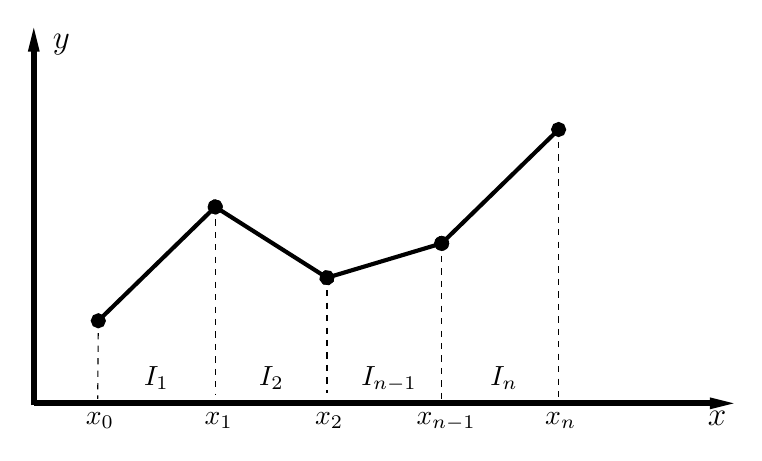
\begin{tikzpicture}[x=0.75pt,y=0.75pt,yscale=-1,xscale=1]
        %uncomment if require: \path (0,292); %set diagram left start at 0, and has height of 292
        
        %Straight Lines [id:da0974477033314256] 
        \draw [line width=2.25]    (160.48,243.82) -- (160.48,67.89) ;
        \draw [shift={(160.48,61.89)}, rotate = 90] [fill={rgb, 255:red, 0; green, 0; blue, 0 }  ][line width=0.08]  [draw opacity=0] (11.52,-2.88) -- (0,0) -- (11.52,2.88) -- cycle    ;
        %Straight Lines [id:da9621180723245395] 
        \draw [line width=2.25]    (160.48,242.82) -- (491.72,242.82) ;
        \draw [shift={(497.72,242.82)}, rotate = 180] [fill={rgb, 255:red, 0; green, 0; blue, 0 }  ][line width=0.08]  [draw opacity=0] (11.52,-2.88) -- (0,0) -- (11.52,2.88) -- cycle    ;
        %Straight Lines [id:da8021543661440511] 
        \draw [line width=1.5]    (191.58,203.05) -- (247.92,148.19) ;
        \draw [shift={(247.92,148.19)}, rotate = 315.76] [color={rgb, 255:red, 0; green, 0; blue, 0 }  ][fill={rgb, 255:red, 0; green, 0; blue, 0 }  ][line width=1.5]      (0, 0) circle [x radius= 2.61, y radius= 2.61]   ;
        \draw [shift={(191.58,203.05)}, rotate = 315.76] [color={rgb, 255:red, 0; green, 0; blue, 0 }  ][fill={rgb, 255:red, 0; green, 0; blue, 0 }  ][line width=1.5]      (0, 0) circle [x radius= 2.61, y radius= 2.61]   ;
        %Straight Lines [id:da968568535514678] 
        \draw [line width=1.5]    (247.92,148.19) -- (301.76,182.31) ;
        \draw [shift={(301.76,182.31)}, rotate = 32.36] [color={rgb, 255:red, 0; green, 0; blue, 0 }  ][fill={rgb, 255:red, 0; green, 0; blue, 0 }  ][line width=1.5]      (0, 0) circle [x radius= 2.61, y radius= 2.61]   ;
        \draw [shift={(247.92,148.19)}, rotate = 32.36] [color={rgb, 255:red, 0; green, 0; blue, 0 }  ][fill={rgb, 255:red, 0; green, 0; blue, 0 }  ][line width=1.5]      (0, 0) circle [x radius= 2.61, y radius= 2.61]   ;
        %Straight Lines [id:da5858741699608034] 
        \draw [line width=1.5]    (357.01,165.76) -- (301.76,182.31) ;
        \draw [shift={(301.76,182.31)}, rotate = 163.33] [color={rgb, 255:red, 0; green, 0; blue, 0 }  ][fill={rgb, 255:red, 0; green, 0; blue, 0 }  ][line width=1.5]      (0, 0) circle [x radius= 2.61, y radius= 2.61]   ;
        \draw [shift={(357.01,165.76)}, rotate = 163.33] [color={rgb, 255:red, 0; green, 0; blue, 0 }  ][fill={rgb, 255:red, 0; green, 0; blue, 0 }  ][line width=1.5]      (0, 0) circle [x radius= 2.61, y radius= 2.61]   ;
        %Straight Lines [id:da9973898432779882] 
        \draw [line width=1.5]    (357.01,165.76) -- (413.35,110.9) ;
        \draw [shift={(413.35,110.9)}, rotate = 315.76] [color={rgb, 255:red, 0; green, 0; blue, 0 }  ][fill={rgb, 255:red, 0; green, 0; blue, 0 }  ][line width=1.5]      (0, 0) circle [x radius= 2.61, y radius= 2.61]   ;
        \draw [shift={(357.01,165.76)}, rotate = 315.76] [color={rgb, 255:red, 0; green, 0; blue, 0 }  ][fill={rgb, 255:red, 0; green, 0; blue, 0 }  ][line width=1.5]      (0, 0) circle [x radius= 2.61, y radius= 2.61]   ;
        %Straight Lines [id:da8399761990779901] 
        \draw  [dash pattern={on 2.25pt off 2.25pt on 2.25pt off 2.25pt}]  (191.58,203.05) -- (191.28,240.71) ;
        %Straight Lines [id:da7055601101038533] 
        \draw  [dash pattern={on 2.25pt off 2.25pt on 2.25pt off 2.25pt}]  (247.92,148.19) -- (247.92,238.87) ;
        %Straight Lines [id:da1488501299340097] 
        \draw  [dash pattern={on 2.25pt off 2.25pt on 2.25pt off 2.25pt}]  (301.76,182.31) -- (301.76,237.95) ;
        %Straight Lines [id:da7734154912681879] 
        \draw  [dash pattern={on 2.25pt off 2.25pt on 2.25pt off 2.25pt}]  (357.01,165.76) -- (357.01,240.81) ;
        %Straight Lines [id:da6519712739359385] 
        \draw  [dash pattern={on 2.25pt off 2.25pt on 2.25pt off 2.25pt}]  (413.35,110.9) -- (413.35,239.79) ;
        
        % Text Node
        \draw (184.3,245.83) node [anchor=north west][inner sep=0.75pt]  [font=\normalsize] [align=left] {$\displaystyle x_{0}$};
        % Text Node
        \draw (241.54,245.8) node [anchor=north west][inner sep=0.75pt]  [font=\normalsize] [align=left] {$\displaystyle x_{1}$};
        % Text Node
        \draw (294.78,245.8) node [anchor=north west][inner sep=0.75pt]  [font=\normalsize] [align=left] {$\displaystyle x_{2}$};
        % Text Node
        \draw (343.66,245.8) node [anchor=north west][inner sep=0.75pt]  [font=\normalsize] [align=left] {$\displaystyle x_{n-1}$};
        % Text Node
        \draw (405.64,245.8) node [anchor=north west][inner sep=0.75pt]  [font=\normalsize] [align=left] {$\displaystyle x_{n}$};
        % Text Node
        \draw (212.42,223.75) node [anchor=north west][inner sep=0.75pt]  [font=\normalsize] [align=left] {$\displaystyle I_{1}$};
        % Text Node
        \draw (267.78,223.8) node [anchor=north west][inner sep=0.75pt]  [font=\normalsize] [align=left] {$\displaystyle I_{2}$};
        % Text Node
        \draw (317.03,223.8) node [anchor=north west][inner sep=0.75pt]  [font=\normalsize] [align=left] {$\displaystyle I_{n-1}$};
        % Text Node
        \draw (379.26,223.8) node [anchor=north west][inner sep=0.75pt]  [font=\normalsize] [align=left] {$\displaystyle I_{n}$};
        % Text Node
        \draw (484.01,245.54) node [anchor=north west][inner sep=0.75pt]  [font=\large] [align=left] {$\displaystyle x$};
        % Text Node
        \draw (168.48,63.69) node [anchor=north west][inner sep=0.75pt]  [font=\large] [align=left] {$\displaystyle y$};
        
        
        \end{tikzpicture}    
        \caption*{Example of a linear spline}   
\end{figure}

\subsubsection*{Quadratic Spline}
If by ``smooth'' we mean with continuous derivative then $f(x)$ could represented by quadratic functions $f_i(x)=a_ix^2+b_ix+c_i$ on each segment $I_i = [x_{i-1}, x_i]$. Moreover, every $f_i(x)$ not only satisfies $f_i(x_{i-1})=y_{i-1}$ and $f_i(x_{i})=y_i$, but also $f_i'(x_{i-1})=f_{i-1}'(x_{i-1})$. Since for $i=1$ last condition does not make sense, we use initial condition\footnote{Usually, for the sake of simplicity, $g(x)$ is set to be $0$ or $x$. However, choice of $g(x)$ depends on subject area. For example, initial condition $g(x)=f_n'(x_n)$ is used for periodic processing.} $f'_1(x_{0}) = g(x)$ instead. 
\newpage

Finally, we have following formulation of the problem~ ~ ~ ~ ~ ~ ~ ~ ~ ~ ~ ~ ~ ~ ~ ~ ~ ~ ~ ~ 
\begin{wrapfigure}[10]{r}{0.55\columnwidth}
    \includegraphics[width=0.55\columnwidth]{lectures/images/quadratic_spline.png}
    \caption*{Example of quadratic spline}
\end{wrapfigure}
\[
    f(x) = 
    \left\{ 
    \begin{array}{l l}
        f_1(x), & x \in I_1\\
        f_2(x), & x \in I_2\\
        \vdots \\
        f_n(x), & x \in I_n
    \end{array}
    \right.,
\]
where $f_i(x)$ satisfies
\[
    \left\{
    \begin{array}{l l}
        f_i(x) = a_ix^2+b_ix+c_i, & \forall i\\
        f_i(x_i) = y_i, & \forall i\\
        f_i(x_{i-1}) = y_{i-1}, & \forall i\\
        f'_i(x_{i-1}) = f'_{i-1}(x_{i-1}), & i>1\\
        f'_1(x_{0}) = g(x), & i=1\\
    \end{array}  
    \right..
\]
Such $f(x)$ we call quadratic spline. 
\\\\
\subsubsection*{Cubic spline}
If by ``smooth'' we mean with third continuous derivative then $f(x)$ could represented by cubic functions $f_i(x)=a_ix^3+b_ix^2+c_ix+d_i$ on each segment $I_i = [x_{i-1}, x_i]$. Moreover, every $f_i(x)$ not only satisfies $f_i(x_{i-1})=y_{i-1}$ and $f_i(x_{i})=y_i$, but also $f_i'(x_{i-1})=f_{i-1}'(x_{i-1})$ and $f_i''(x_{i-1})=f_{i-1}''(x_{i-1})$. Since for $i=1$ last conditions does not make sense, we use initial conditions $f'_1(x_{0}) = g_1(x)$ and $f''_1(x_{0}) = g_1(x)$ instead. 
\[
    f(x) = 
    \left\{ 
    \begin{array}{l l}
        f_1(x), & x \in I_1\\
        f_2(x), & x \in I_2\\
        \vdots \\
        f_n(x), & x \in I_n
    \end{array}
    \right.,
\]
where $f_i(x)$ satisfies
\[
    \left\{
    \begin{array}{l l}
        f_i(x) = a_ix^2+b_ix+c_i, & \forall i\\
        f_i(x_i) = y_i, & \forall i\\
        f_i(x_{i-1}) = y_{i-1}, & \forall i\\
        f'_i(x_{i-1}) = f'_{i-1}(x_{i-1}), & i>1\\
        f''_i(x_{i-1}) = f''_{i-1}(x_{i-1}), & i>1\\
        f'_1(x_{0}) = g_1(x), & i=1\\
        f''_1(x_{0}) = g_2(x), & i=1
    \end{array}  
    \right..
\]
Such $f(x)$ we call cubic spline. 
\newpage
\subsection*{Bézier curves}

 A Bézier curve\footnote{The Bézier curve is named after French engineer Pierre Bézier (1910–1999), who used it in the 1962 for designing curves for the bodywork of Renault cars. The method developed first developed in 1959 by Paul de Casteljau for Citroen cars. However, at the time Paul de Casteljau could not publish his works} is a parametric curve used in computer graphics and related fields. A set of discrete "control points" defines a smooth, continuous curve by means of a formula. Usually the curve is intended to approximate a real-world shape that otherwise has no mathematical representation or whose representation is unknown or too complicated. 
 
Bézier curve interpolation problem is formulated as follows. Given a set of control points $P_0,~P_1,~\ldots,~P_n~\in~\R^m$ approximate the path $P_0 \to P_1 \to P_2 \to \ldots \to P_n$ by a smooth parametric curve $B(t)$. Number of  control points $n$ is called degree of a Bézier curve. We denote  Bézier curve that approximate $k$ control points $P_0,~P_1,~\ldots,~P_k~\in~\R^m$ by $B_{{P}_{0}{P}_{1}\ldots{P}_{k}}(t)$.
\begin{figure}[H]
    \centering
    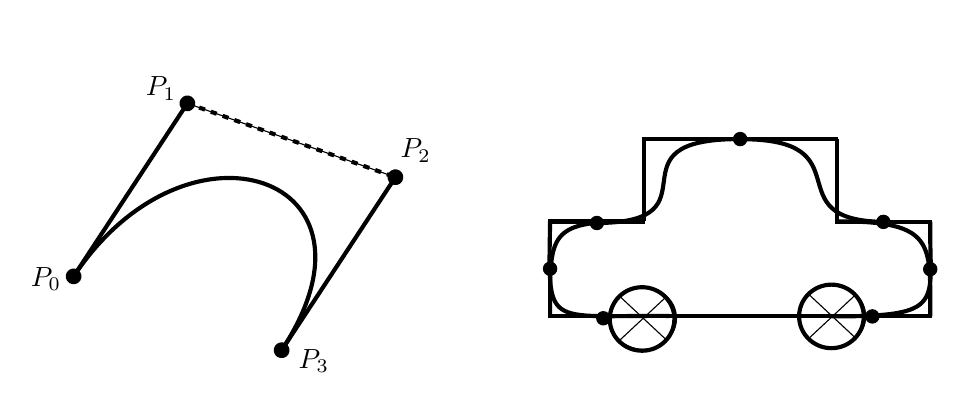
\begin{tikzpicture}[x=0.75pt,y=0.75pt,yscale=-0.8,xscale=0.8]
        %uncomment if require: \path (0,300); %set diagram left start at 0, and has height of 300
        
        %Straight Lines [id:da38433525072365593] 
        \draw [line width=1.5]    (85.33,195.15) -- (128.08,130.14) -- (153.85,90.94) ;
        \draw [shift={(153.85,90.94)}, rotate = 303.33] [color={rgb, 255:red, 0; green, 0; blue, 0 }  ][fill={rgb, 255:red, 0; green, 0; blue, 0 }  ][line width=1.5]      (0, 0) circle [x radius= 3.48, y radius= 3.48]   ;
        \draw [shift={(85.33,195.15)}, rotate = 303.33] [color={rgb, 255:red, 0; green, 0; blue, 0 }  ][fill={rgb, 255:red, 0; green, 0; blue, 0 }  ][line width=1.5]      (0, 0) circle [x radius= 3.48, y radius= 3.48]   ;
        %Straight Lines [id:da29504840381981623] 
        \draw [line width=1.5]    (210.61,239.62) -- (253.36,174.61) -- (279.13,135.42) ;
        \draw [shift={(279.13,135.42)}, rotate = 303.33] [color={rgb, 255:red, 0; green, 0; blue, 0 }  ][fill={rgb, 255:red, 0; green, 0; blue, 0 }  ][line width=1.5]      (0, 0) circle [x radius= 3.48, y radius= 3.48]   ;
        \draw [shift={(210.61,239.62)}, rotate = 303.33] [color={rgb, 255:red, 0; green, 0; blue, 0 }  ][fill={rgb, 255:red, 0; green, 0; blue, 0 }  ][line width=1.5]      (0, 0) circle [x radius= 3.48, y radius= 3.48]   ;
        %Curve Lines [id:da5407723730641252] 
        \draw [line width=1.5]    (85.33,195.15) .. controls (153.78,91.87) and (280.19,134.32) .. (210.61,239.62) ;
        %Straight Lines [id:da23030185871120712] 
        \draw [line width=1.5]  [dash pattern={on 2.25pt off 2.25pt on 2.25pt off 2.25pt}]  (153.85,90.94) -- (279.13,135.42) ;
        %Straight Lines [id:da5340691028310462] 
        \draw    (153.85,90.94) -- (279.13,135.42) ;
        %Straight Lines [id:da8521843013648231] 
        \draw    (372.28,162.07) -- (372.28,218.99) ;
        %Straight Lines [id:da0295218077708157] 
        \draw [line width=1.5]    (371.27,162.07) -- (429.67,162.07) ;
        %Straight Lines [id:da5061662479170574] 
        \draw [line width=1.5]    (428.63,112.52) -- (428.63,162.07) ;
        %Straight Lines [id:da35589500200732105] 
        \draw [line width=1.5]    (371.27,218.99) -- (602.27,218.99) ;
        %Straight Lines [id:da38216385176759493] 
        \draw [line width=1.5]    (427.67,112.52) -- (545.97,112.52) ;
        %Straight Lines [id:da6550091589363698] 
        \draw [line width=1.5]    (544.88,112.52) -- (544.88,162.33) ;
        %Straight Lines [id:da6587237439435061] 
        \draw [line width=1.5]    (543.87,162.33) -- (602.17,162.33) ;
        %Straight Lines [id:da7485059129149993] 
        \draw    (601.22,162.33) -- (601.22,219.25) ;
        %Curve Lines [id:da15087650946616193] 
        \draw [line width=1.5]    (372.28,218.99) .. controls (372.37,168.83) and (369.49,161.15) .. (428.63,162.07) ;
        %Curve Lines [id:da6302009599851996] 
        \draw [line width=1.5]    (372.28,162.07) .. controls (371.33,227.47) and (367.87,218.41) .. (443.99,218.97) ;
        %Shape: Ellipse [id:dp7231329766860946] 
        \draw  [line width=1.5]  (408.22,220.79) .. controls (408.22,210.23) and (416.94,201.66) .. (427.69,201.66) .. controls (438.44,201.66) and (447.15,210.23) .. (447.15,220.79) .. controls (447.15,231.36) and (438.44,239.92) .. (427.69,239.92) .. controls (416.94,239.92) and (408.22,231.36) .. (408.22,220.79) -- cycle ;
        %Curve Lines [id:da6611347177881066] 
        \draw [line width=1.5]    (544.67,162) .. controls (604.94,161.68) and (601.12,175.61) .. (601.22,219.25) ;
        %Curve Lines [id:da3691402467708471] 
        \draw [line width=1.5]    (541.73,219.25) .. controls (612.08,219.25) and (600.54,211.88) .. (601.22,162.33) ;
        %Shape: Ellipse [id:dp5936137420517733] 
        \draw  [line width=1.5]  (522.26,219.25) .. controls (522.26,208.68) and (530.98,200.12) .. (541.73,200.12) .. controls (552.48,200.12) and (561.19,208.68) .. (561.19,219.25) .. controls (561.19,229.81) and (552.48,238.38) .. (541.73,238.38) .. controls (530.98,238.38) and (522.26,229.81) .. (522.26,219.25) -- cycle ;
        %Curve Lines [id:da5823575046185543] 
        \draw [line width=1.5]    (400.46,163) .. controls (476.13,162.58) and (403.73,112.18) .. (486.75,112.45) ;
        %Curve Lines [id:da8670088232112763] 
        \draw [line width=1.5]    (486.75,112.52) .. controls (563.33,112.18) and (506.13,161.38) .. (573.05,162.33) ;
        %Flowchart: Summing Junction [id:dp9099421329485471] 
        \draw   (408.34,220.37) .. controls (408.34,210.04) and (417.31,201.66) .. (428.38,201.66) .. controls (439.45,201.66) and (448.42,210.04) .. (448.42,220.37) .. controls (448.42,230.7) and (439.45,239.08) .. (428.38,239.08) .. controls (417.31,239.08) and (408.34,230.7) .. (408.34,220.37) -- cycle ; \draw   (414.21,207.14) -- (442.55,233.6) ; \draw   (442.55,207.14) -- (414.21,233.6) ;
        %Flowchart: Summing Junction [id:dp8125787866129444] 
        \draw   (522.26,219.25) .. controls (522.26,208.91) and (531.23,200.54) .. (542.3,200.54) .. controls (553.37,200.54) and (562.34,208.91) .. (562.34,219.25) .. controls (562.34,229.58) and (553.37,237.95) .. (542.3,237.95) .. controls (531.23,237.95) and (522.26,229.58) .. (522.26,219.25) -- cycle ; \draw   (528.13,206.02) -- (556.47,232.47) ; \draw   (556.47,206.02) -- (528.13,232.47) ;
        %Shape: Circle [id:dp9125474207316695] 
        \draw  [fill={rgb, 255:red, 0; green, 0; blue, 0 }  ,fill opacity=1 ] (368.28,190.53) .. controls (368.28,188.32) and (370.07,186.53) .. (372.28,186.53) .. controls (374.49,186.53) and (376.28,188.32) .. (376.28,190.53) .. controls (376.28,192.74) and (374.49,194.53) .. (372.28,194.53) .. controls (370.07,194.53) and (368.28,192.74) .. (368.28,190.53) -- cycle ;
        %Shape: Circle [id:dp9953749827310527] 
        \draw  [fill={rgb, 255:red, 0; green, 0; blue, 0 }  ,fill opacity=1 ] (396.46,163) .. controls (396.46,160.79) and (398.25,159) .. (400.46,159) .. controls (402.66,159) and (404.46,160.79) .. (404.46,163) .. controls (404.46,165.21) and (402.66,167) .. (400.46,167) .. controls (398.25,167) and (396.46,165.21) .. (396.46,163) -- cycle ;
        %Shape: Circle [id:dp6374702071737668] 
        \draw  [fill={rgb, 255:red, 0; green, 0; blue, 0 }  ,fill opacity=1 ] (482.75,112.45) .. controls (482.75,110.24) and (484.55,108.45) .. (486.75,108.45) .. controls (488.96,108.45) and (490.75,110.24) .. (490.75,112.45) .. controls (490.75,114.66) and (488.96,116.45) .. (486.75,116.45) .. controls (484.55,116.45) and (482.75,114.66) .. (482.75,112.45) -- cycle ;
        %Shape: Circle [id:dp35980495806930546] 
        \draw  [fill={rgb, 255:red, 0; green, 0; blue, 0 }  ,fill opacity=1 ] (569.02,162.33) .. controls (569.02,160.12) and (570.81,158.33) .. (573.02,158.33) .. controls (575.23,158.33) and (577.02,160.12) .. (577.02,162.33) .. controls (577.02,164.54) and (575.23,166.33) .. (573.02,166.33) .. controls (570.81,166.33) and (569.02,164.54) .. (569.02,162.33) -- cycle ;
        %Shape: Circle [id:dp23695820368705234] 
        \draw  [fill={rgb, 255:red, 0; green, 0; blue, 0 }  ,fill opacity=1 ] (562.34,219.25) .. controls (562.34,217.04) and (564.13,215.25) .. (566.34,215.25) .. controls (568.55,215.25) and (570.34,217.04) .. (570.34,219.25) .. controls (570.34,221.46) and (568.55,223.25) .. (566.34,223.25) .. controls (564.13,223.25) and (562.34,221.46) .. (562.34,219.25) -- cycle ;
        %Shape: Circle [id:dp9552208675934684] 
        \draw  [fill={rgb, 255:red, 0; green, 0; blue, 0 }  ,fill opacity=1 ] (597.22,190.79) .. controls (597.22,188.58) and (599.02,186.79) .. (601.22,186.79) .. controls (603.43,186.79) and (605.22,188.58) .. (605.22,190.79) .. controls (605.22,193) and (603.43,194.79) .. (601.22,194.79) .. controls (599.02,194.79) and (597.22,193) .. (597.22,190.79) -- cycle ;
        %Shape: Circle [id:dp6707745479541134] 
        \draw  [fill={rgb, 255:red, 0; green, 0; blue, 0 }  ,fill opacity=1 ] (400.34,220.37) .. controls (400.34,218.16) and (402.13,216.37) .. (404.34,216.37) .. controls (406.55,216.37) and (408.34,218.16) .. (408.34,220.37) .. controls (408.34,222.58) and (406.55,224.37) .. (404.34,224.37) .. controls (402.13,224.37) and (400.34,222.58) .. (400.34,220.37) -- cycle ;
        
        % Text Node
        \draw (201.57,53) node   [align=left] {\begin{minipage}[lt]{88.27pt}
        \end{minipage}};
        % Text Node
        \draw (489.57,61.97) node   [align=left] {\begin{minipage}[lt]{88.27pt} 
        \end{minipage}};
        % Text Node
        \draw (127.33,73.47) node [anchor=north west][inner sep=0.75pt]   [align=left] {$\displaystyle P_{1}$};
        % Text Node
        \draw (280.67,110.8) node [anchor=north west][inner sep=0.75pt]   [align=left] {$\displaystyle P_{2}$};
        % Text Node
        \draw (58,188.13) node [anchor=north west][inner sep=0.75pt]   [align=left] {$\displaystyle P_{0}$};
        % Text Node
        \draw (219.33,237.47) node [anchor=north west][inner sep=0.75pt]   [align=left] {$\displaystyle P_{3}$};
        \end{tikzpicture}        
    \caption*{\small Examples of Bézier curves}    
\end{figure}
\begin{theorema}{Recursive formula for Bézier curve}{}
    Bézier curve ${B}(t)$ could be find using following recursive formula
    \begin{eqnarray}
    {B} _{{P} _{0}}(t)&=&{P} _{0}, \ t\in[0,1].\nonumber\\
    {B} _{{P} _{0}{P} _{1}\ldots {P} _{k}}(t)&=&(1-t){B}_{{P}_{0}{P}_{k}\ldots {P}_{n-1}}(t)+t{B} _{{P} _{1}{P} _{2}\ldots {P}_{n}}(t), \ t\in[0,1].\nonumber
    \end{eqnarray}
\end{theorema}
\Ex Given a set of control points $P_0,~P_1~\in~\R^m$ approximate the path $P_0 \to P_1$ by a smooth parametric curve $B(t)$. Using recursive formula for Bézier curve, we get
\begin{eqnarray}
    B_{P_{0}}(t)&=&P_{0},\nonumber\\
    B_{P_{1}}(t)&=&P_{1},\nonumber\\
    B(t)&=&B_{P_{0}P_{1}}(t)=(1-t)B_{P_{0}}+tB_{P_{1}}=(1-t)P_{0}+tP_{1}.\nonumber
\end{eqnarray}
\begin{theorema}{Explicit formula for Bézier curve}{}
Bézier curve ${B}(t)$ could be find using following explicit formula
\[
    B(t) = \sum\limits_{i=0}^n P_i \cdot b_{n,i}(t),  
\]
where $b_{n,i}$ are Bernstein polynomials of a form
\[
    b_{n,i} = C_n^i (1-t)^{n-i}t^i.
\]
\end{theorema}
